\everymath{\displaystyle}
\documentclass{beamer}
% \documentclass[handout]{beamer}

%\usepackage[pdftex]{color,graphicx}
\usepackage{amsmath,amssymb,amsfonts}

\mode<presentation>
{
  % \usetheme{Darmstadt}
  % \usetheme[hideothersubsections]{Hannover}
  % \usetheme[hideothersubsections]{Goettingen}
  \usetheme[hideothersubsections, right]{Berkeley}

  \usecolortheme{seahorse}
  % \usecolortheme{dolphin}
  \usecolortheme{rose}
  % \usecolortheme{orchid}

  \useinnertheme[shadow]{rounded}

  \setbeamercovered{transparent}
  % or whatever (possibly just delete it)
}

\mode<handout>{
  \setbeamercolor{background canvas}{bg=black!5}
  \usepackage{pgfpages}
  \pgfpagesuselayout{4 on 1}[a4paper,border shrink=5mm, landscape]
}

\usepackage[brazilian]{babel}
% or whatever

% \usepackage[latin1]{inputenc}
\usepackage[utf8]{inputenc}
% or whatever

\usepackage{times}
%\usepackage[T1]{fontenc}
% Or whatever. Note that the encoding and the font should match. If T1
% does not look nice, try deleting the line with the fontenc.


\title%[] % (optional, use only with long paper titles)
{Tópicos de busca bibliográfica}

\subtitle
{Google-fu et al} % (optional)

\author%[] % (optional, use only with lots of authors)
{Felipe Figueiredo}% \and S.~Another\inst{2}}
% - Use the \inst{?} command only if the authors have different
%   affiliation.

\institute[INTO] % (optional, but mostly needed)
{Instituto Nacional de Traumatologia e Ortopedia
}
  % \inst{1}%
  % Department of Computer Science\\
  % University of Somewhere
  % \and
  % \inst{2}%
  % Department of Theoretical Philosophy\\
  % University of Elsewhere}
% - Use the \inst command only if there are several affiliations.
% - Keep it simple, no one is interested in your street address.

\date%[] % (optional)
{}

% \subject{Talks}
% This is only inserted into the PDF information catalog. Can be left
% out. 



% If you have a file called "university-logo-filename.xxx", where xxx
% is a graphic format that can be processed by latex or pdflatex,
% resp., then you can add a logo as follows:

\pgfdeclareimage[height=1.6cm]{university-logo}{../logo}
\logo{\pgfuseimage{university-logo}}



% Delete this, if you do not want the table of contents to pop up at
% the beginning of each subsection:
\AtBeginSubsection[]
%\AtBeginSection[]
{
  \begin{frame}<beamer>{Sumário}
    \tableofcontents[currentsection,currentsubsection]
  \end{frame}
}


% If you wish to uncover everything in a step-wise fashion, uncomment
% the following command: 

\beamerdefaultoverlayspecification{<+->}


\begin{document}

\begin{frame}
  \titlepage
\end{frame}

\begin{frame}{Sumário}
  \tableofcontents
  % You might wish to add the option [pausesections]
\end{frame}


%% Template
% \section{}

% \subsection{}

% \begin{frame}{}
%   \begin{itemize}
%   \item 
%   \end{itemize}
% \end{frame}

% \begin{frame}
%   \begin{columns}
%     \begin{column}{5cm}
%     \end{column}
%     \begin{column}{5cm}
%     \end{column}
%   \end{columns}
% \end{frame}

% \begin{frame}{}
%   \includegraphics[height=0.4\textheight]{file1}
%   \includegraphics[height=0.4\textheight]{file2}
%   \includegraphics[height=0.4\textheight]{file3}
%   \begin{figure}
%     \caption{}
%   \end{figure}
% \end{frame}

% \begin{frame}{}
%   \begin{definition}
%   \end{definition}
%   \begin{example}
%   \end{example}
%   \begin{block}{Exercício}
%   \end{block}
% \end{frame}

\section{Bases bibliográficas}

\begin{frame}{Bases bibliográficas na Internet}
  \begin{itemize}
  \item Antigamente localizava-se livros e revistas por fichas nas
    bibliotecas (papel!)
  \item Hoje podemos fazer buscas profundas em bases bibliográficas
    (conteúdo completo das obras)
  \end{itemize}
\end{frame}

\begin{frame}{Exemplos}
  \begin{itemize}
  \item \alert{PUBMED} - \url{www.pubmed.org} (ou .com)
  \item \alert{PubMed Central} - \url{www.ncbi.nlm.nih.gov/pmc/}
  \item \alert{Google Scholar} - \url{scholar.google.com}
  \item<4-> Web of Science - \url{www.webofknowledge.com}
  \item<4-> Scielo - \url{www.scielo.br}
  \item<4-> CrossRef - \url{www.crossref.org}
  \item<4-> etc\ldots
  \end{itemize}
\end{frame}

\subsection{PUBMED e PubMed Central}

\begin{frame}{PUBMED}
  \begin{itemize}
  \item \alert{Mecanismo de busca}, mantido pelo governo dos EUA
    (NLM\footnote{National Library of Medicine} e
    NIH\footnote{National Institutes of Health})
  \item Acessa primariamente a base MEDLINE, entre outras
  \item Referências dos artigos são indexadas e catalogadas para busca
  \item Links para o conteúdo dos artigos (externos)
  \item Sugere artigos similares
  \item Exporta referências para gerenciadores (Mendeley, EndNote, etc)
  \end{itemize}
\end{frame}

\begin{frame}{MEDLINE}
  \begin{definition}
    Base bibliográfica de acesso gratuito de referências de Ciências
    da Saúde e afins
  \end{definition}
  Disponíveis:
  \begin{itemize}
  \item Índice
  \item Abstract
  \item Link para artigo completo (em geral, site da editora)
  \end{itemize}
\end{frame}

\begin{frame}{MEDLINE (escopo)}
  \begin{block}{De acordo com a Wikipédia}
    Disciplinas: Medicine, nursing, pharmacy, dentistry, veterinary
    medicine, health care, biology, biochemistry, molecular evolution,
    biomedicine, history of medicine, health services research, AIDS,
    toxicology and environmental health, molecular biology,
    complementary medicine, behavioral sciences, chemical sciences,
    bioengineering, health policy development, environmental science,
    marine biology, plant and animal science, biophysics
  \end{block}
\end{frame}

\begin{frame}{PubMed Central (PMC)}
  \begin{definition}
    Repositório gratuito de artigos Open-Access
  \end{definition}
  Disponíveis:
  \begin{itemize}
  \item Índice
  \item Abstract
  \item Conteúdo integral
  \end{itemize}
\end{frame}

\begin{frame}{PUBMED Busca}
  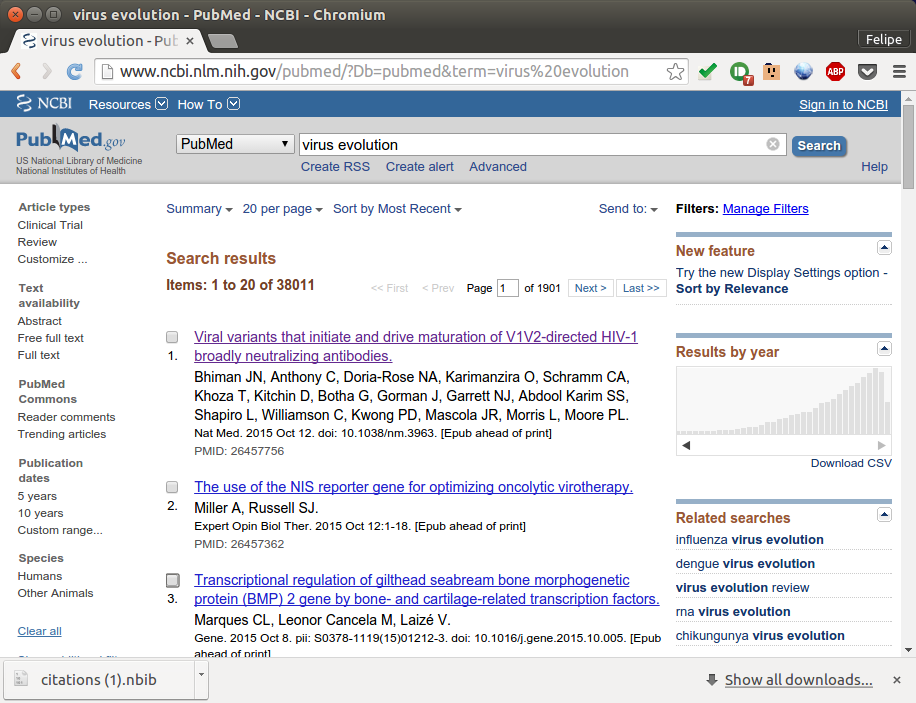
\includegraphics[height=.85\textheight]{Busca/pubmed-busca}
\end{frame}

\begin{frame}{PUBMED Artigo}
  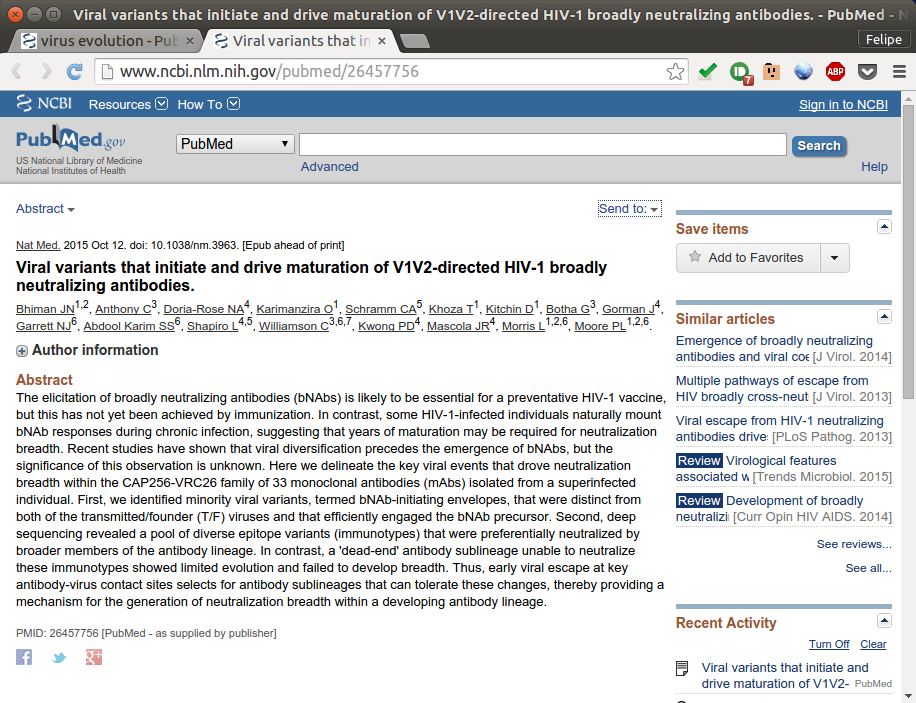
\includegraphics[height=.85\textheight]{Busca/pubmed-paper}
\end{frame}

\begin{frame}{PUBMED Exportando a referência}
  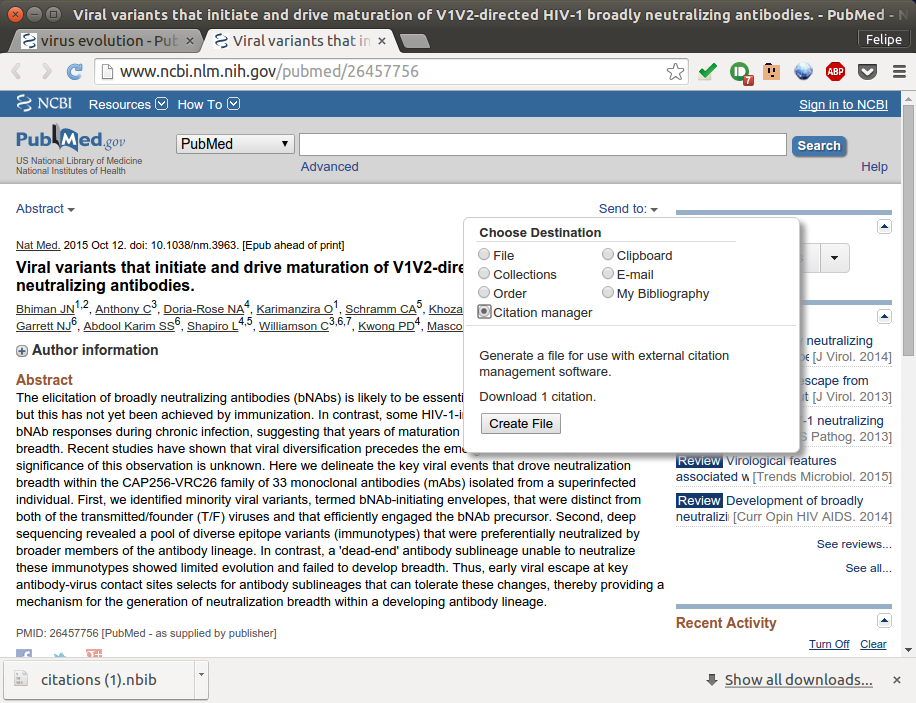
\includegraphics[height=.85\textheight]{Busca/pubmed-export1}
\end{frame}

\begin{frame}{PUBMED Exportando várias referências}
  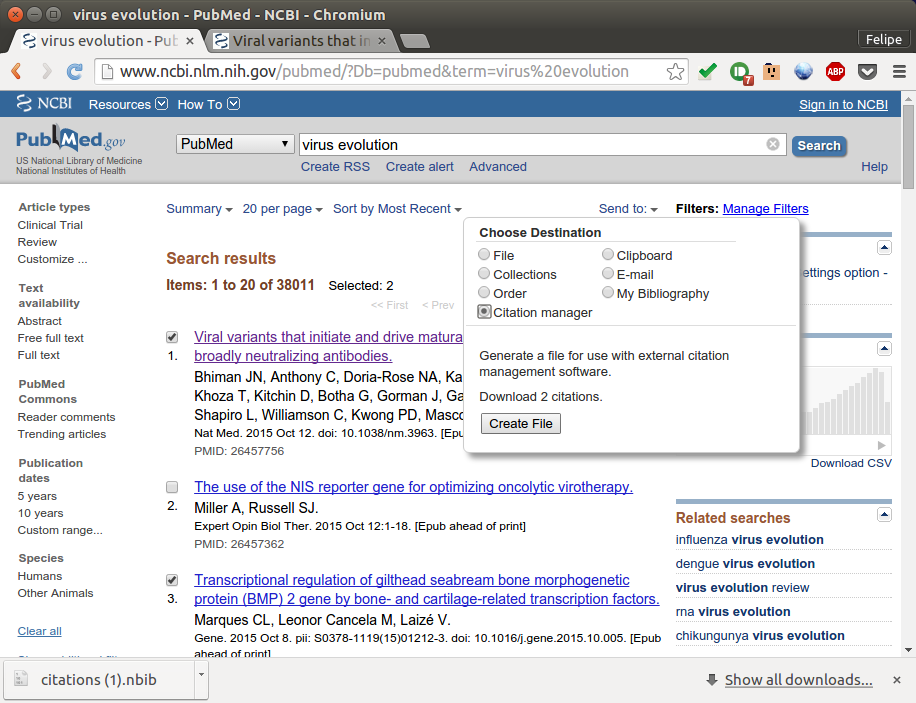
\includegraphics[height=.85\textheight]{Busca/pubmed-export2}
\end{frame}

\subsection{Google Scholar}

\begin{frame}{Google Scholar}
  \begin{definition}
    Mecanismo de busca que acessa a base bibliográfica do Google para
    livros e artigos acadêmicos.
  \end{definition}
  \begin{itemize}
  \item Escopo: A vida, o universo e tudo o mais\footnote{e obrigado
      pelo peixe}
  \item Indexa citações
  \item Facilita acesso ao PDF, caso disponível publicamente
  \item Exporta referências
  \end{itemize}
\end{frame}

\begin{frame}{Google Scholar Busca}
  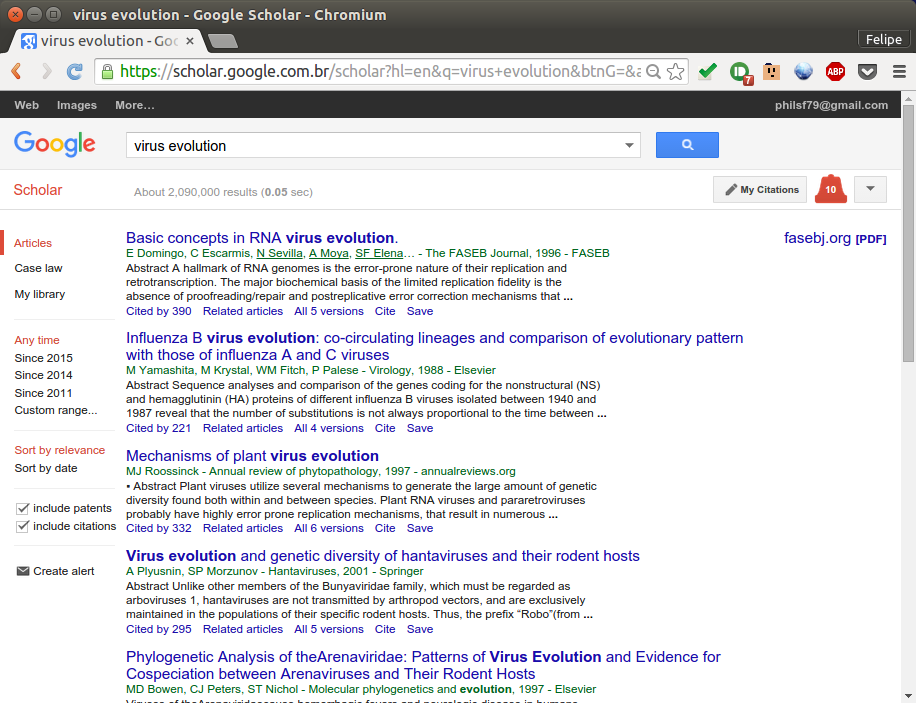
\includegraphics[height=.85\textheight]{Busca/scholar-busca1}
\end{frame}

\begin{frame}{Google Scholar Busca}
  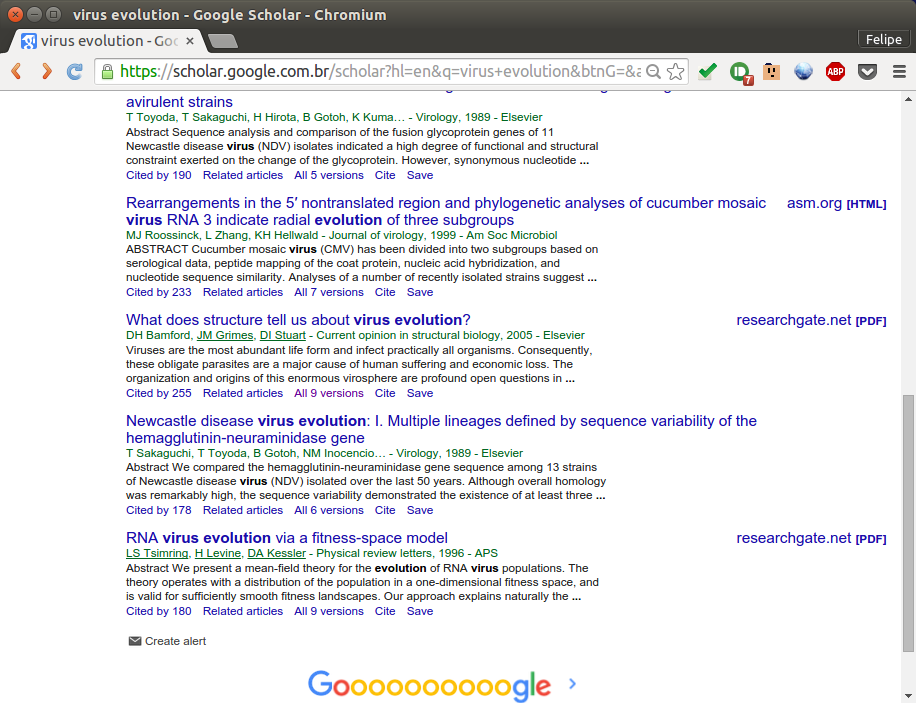
\includegraphics[height=.85\textheight]{Busca/scholar-busca2}
\end{frame}

\begin{frame}{Google Scholar Artigo (todas as versões)}
  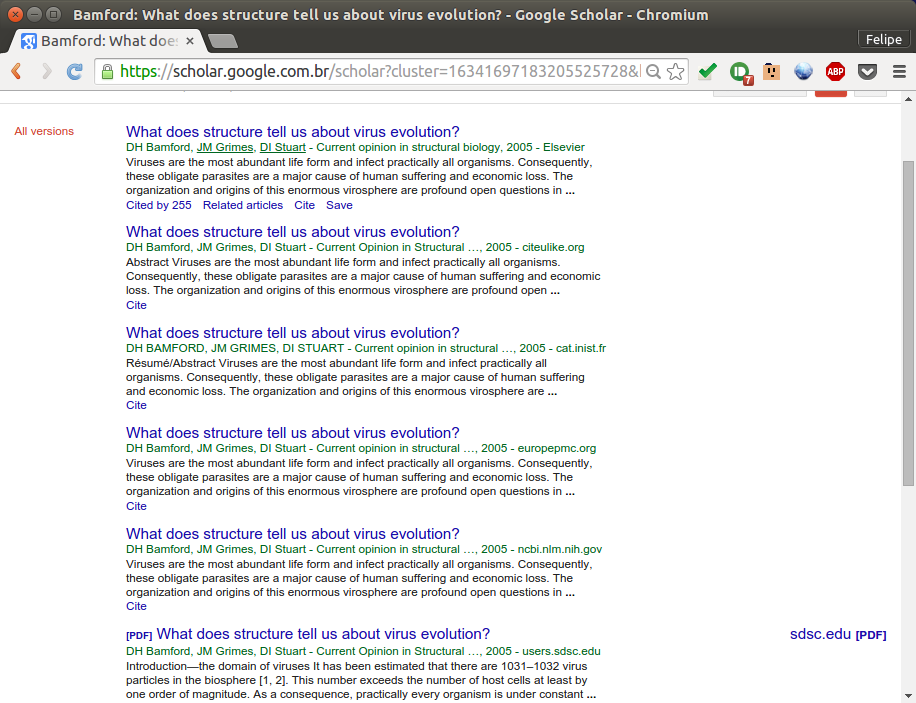
\includegraphics[height=.85\textheight]{Busca/scholar-paper}
\end{frame}

\begin{frame}{Google Scholar Exportando a Referência}
  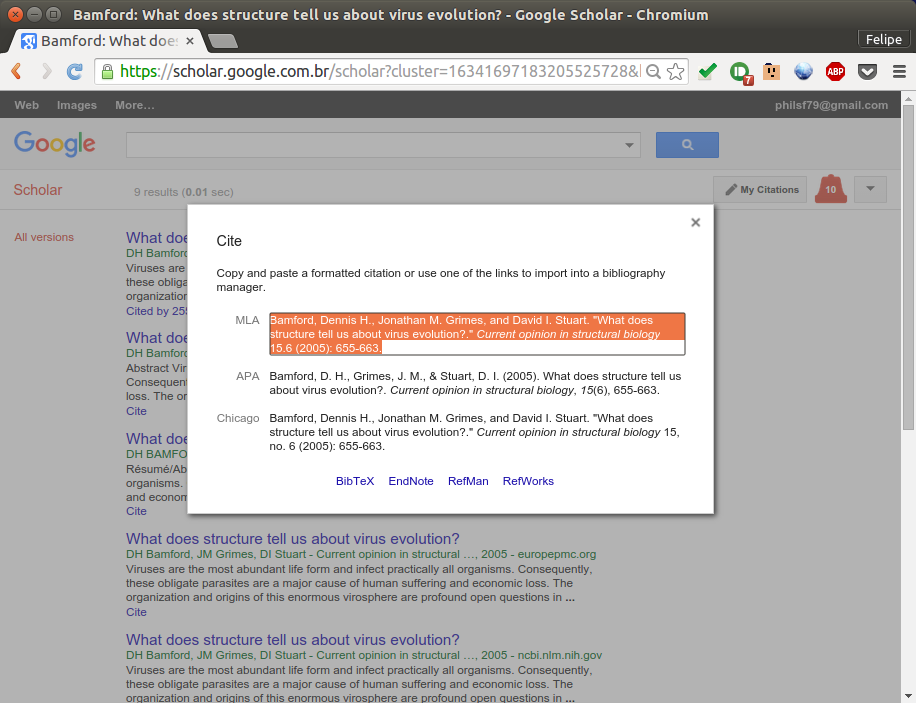
\includegraphics[height=.85\textheight]{Busca/scholar-export}
\end{frame}

\section{Google-fu}

\begin{frame}{Google-fu}
  \begin{block}{Google-fu}
    Habilidade em usar mecanismos de busca (em especial o Google) para
    localizar rapidamente informação na Internet.

    \bigskip
    Referência ao termo {\em kung fu}, cujo domínio exige muita
    dedicação.
  \end{block}
  Fonte: \url{http://english.stackexchange.com/questions/19967/what-does-google-fu-mean}

  \begin{block}{Resumindo}
    Conjunto de técnicas ``avançadas'' usadas quando a informação
    necessária é difícil de ser localizada.
  \end{block}
\end{frame}

\subsection{Opções avançadas de busca}

\begin{frame}{Opções de busca}
  Podemos ampliar ou reduzir o escopo da busca \ldots
  \begin{itemize}
  \item Incluindo obrigatoriamente uma chave de busca (operador +)
  \item Excluindo uma chave de busca (operador -)
  \item Buscando uma frase exata (frase entre aspas)
  \item Combinando todas as opções acima (e outras!)
  \end{itemize}
\end{frame}

\begin{frame}{Busca básica}
  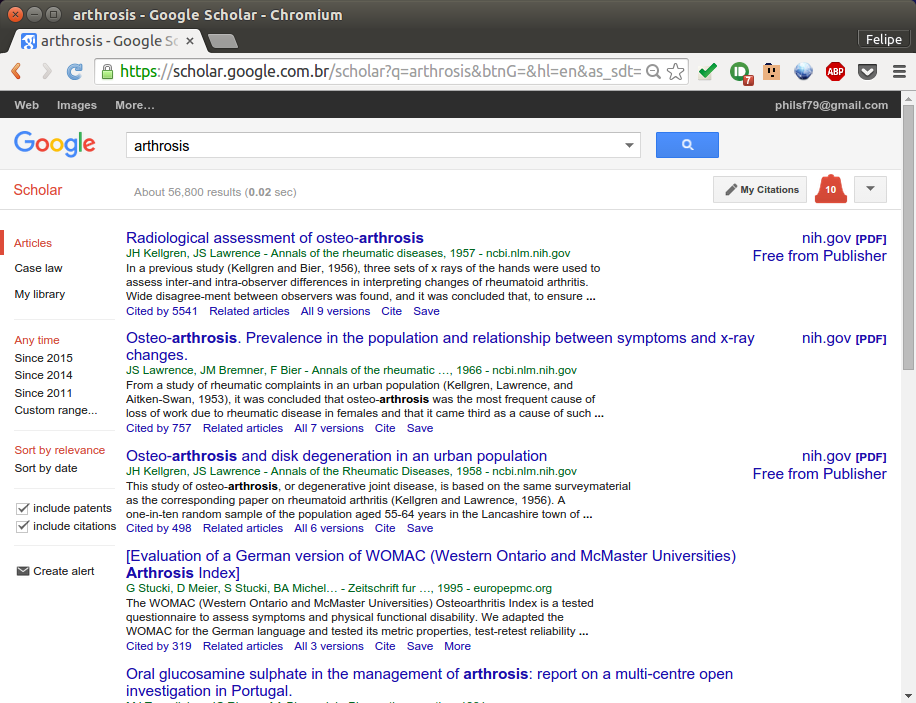
\includegraphics[height=.85\textheight]{Busca/google-fu-basico}
\end{frame}

\begin{frame}{Operador +}
  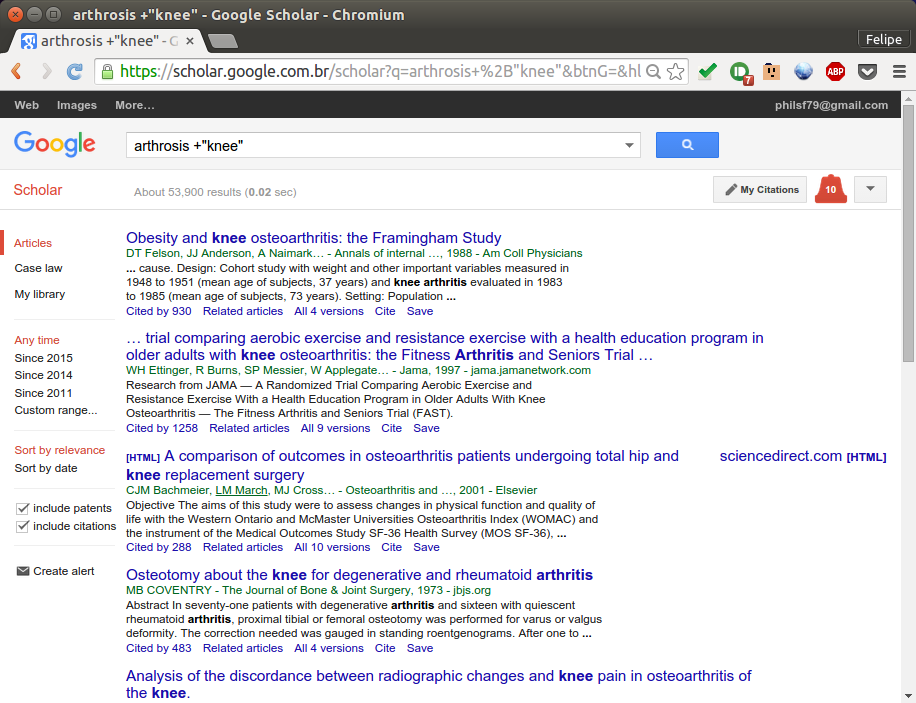
\includegraphics[height=.85\textheight]{Busca/google-fu-plus}
\end{frame}

\begin{frame}{Operador -}
  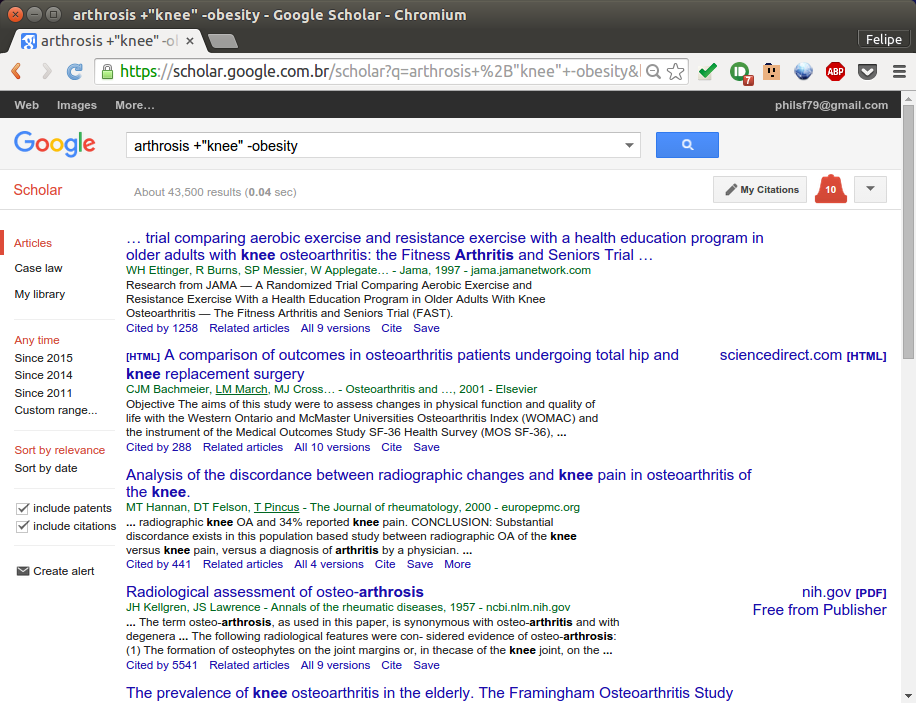
\includegraphics[height=.85\textheight]{Busca/google-fu-plusminus}
\end{frame}

\begin{frame}{Observações}
  \begin{itemize}
  \item Observe que no último exemplo, {\em obesity} foi usada sem
    aspas
  \item Isso significa que o Google não vai procurar a palavra
    \alert{exata}, mas também algumas flexões da mesma
  \end{itemize}
  \begin{example}
    obesity, obese, \ldots
  \end{example}
\end{frame}

\subsection{Google Books}

\begin{frame}{Google Books}
  \begin{itemize}
  \item Plataforma \alert{Google
      Books}\footnote{\url{https://books.google.com/}} (antes: Google
    Book Search e Google Print)
  \item Iniciado em 2004, digitalizou milhões de livros + OCR para
    extrair a íntegra do texto
  \item Tem 4 níveis de acesso para o acervo:
    \begin{enumerate}
    \item Full view (domínio público)
    \item Preview (\% disponível, escolha da editora)
    \item Snippet view (2--3 linhas em torno da chave de busca)
    \item No preview
    \end{enumerate}
  \end{itemize}
\end{frame}

\begin{frame}{Buscando livros no Google Books}
  Pode-se \ldots
  \begin{itemize}
  \item localizar livros buscando por:
    \begin{itemize}
    \item Metadados (autor(es) e/ou título)
    \item Trechos ou frases
    \end{itemize}
  \item consultar preview ou a íntegra (se disponível em domínio
    público)
  \item \alert{exportar} informações bibliográficas\footnote{arquivo
      .RIS} para \alert{importação} no Mendeley (\ldots, Endnote,
    etc.)
  \end{itemize}
\end{frame}

\begin{frame}{Busca por metadados}
  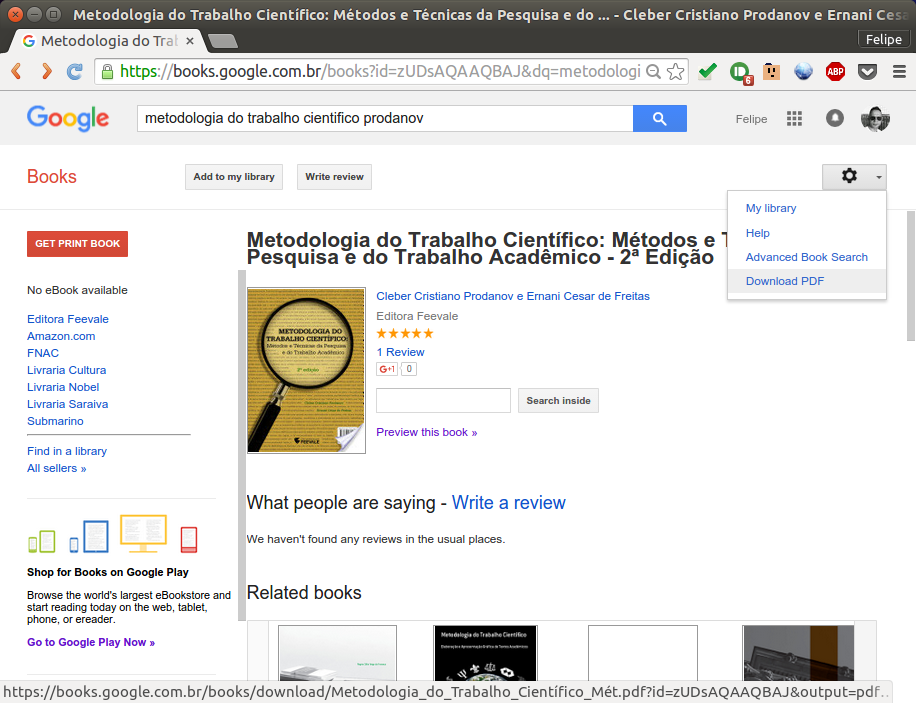
\includegraphics[height=.85\textheight]{Busca/gbooks-livro}

\end{frame}

\begin{frame}{Preview}
  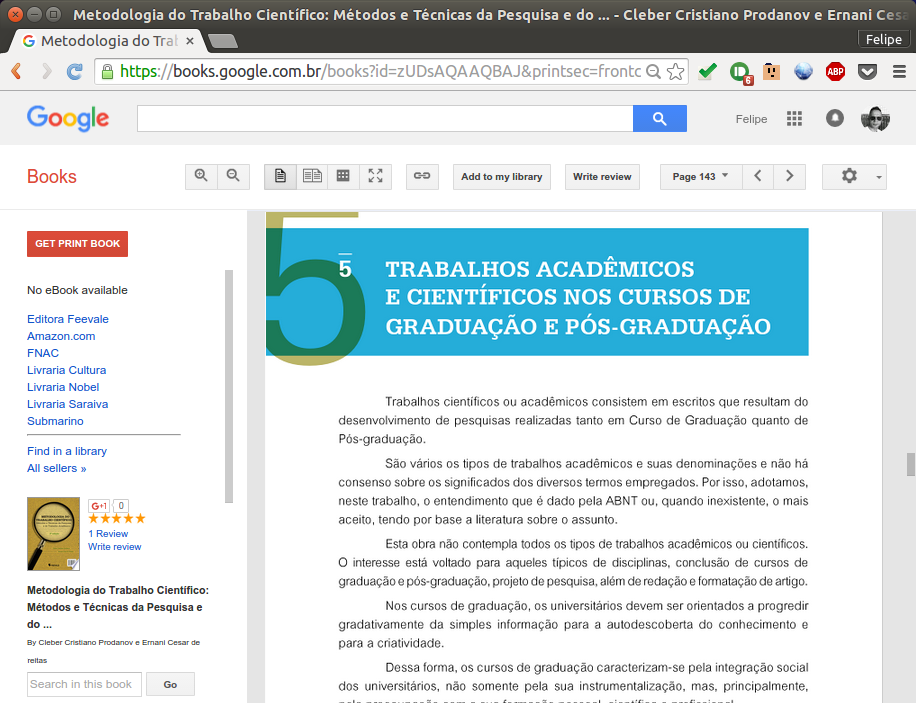
\includegraphics[height=.85\textheight]{Busca/gbooks-preview}
\end{frame}

\begin{frame}{Domínio Público}
  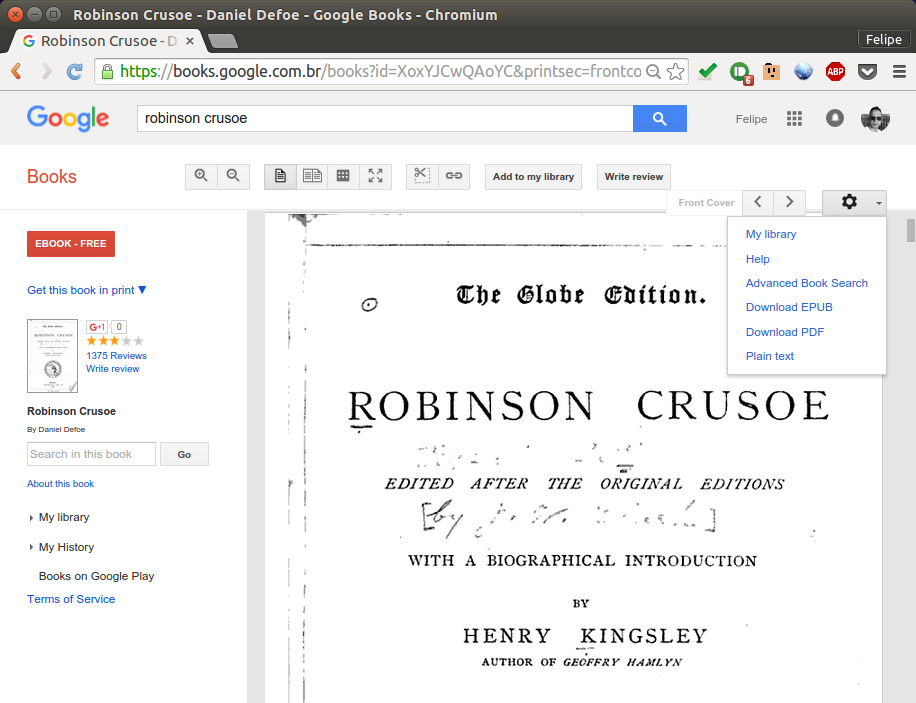
\includegraphics[height=.85\textheight]{Busca/gbooks-publicdomain}
\end{frame}

\begin{frame}{Livros acadêmicos}
  \begin{itemize}
  \item Estamos interessados em livros acadêmicos/científicos
  \item Ao fazer, e.g., uma citação direta, podemos usar o Google
    Books para:
    \begin{itemize}
    \item localizar o livro
    \item importar a referência para nosso gerenciador de refs
    \end{itemize}
  \end{itemize}
  \begin{example}[Buscando a frase\ldots]
    ``Life depends on the ability of cells to store, retrieve, and
    translate the genetic instructions required to make and maintain a
    living organism.''
  \end{example}
\end{frame}

\begin{frame}{Busca por conteúdo}
  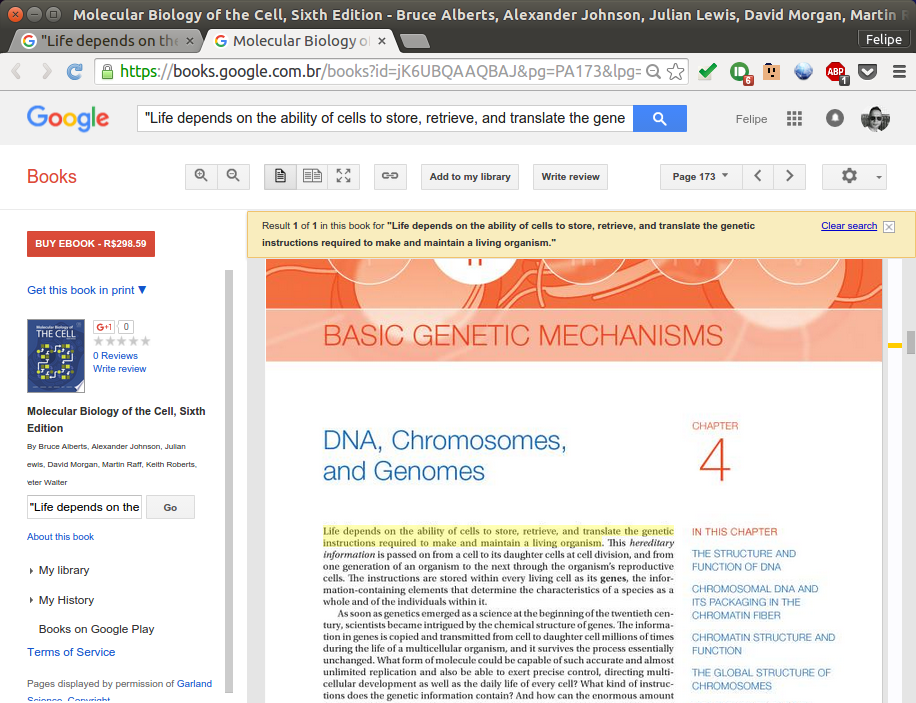
\includegraphics[height=.85\textheight]{Busca/gbooks-busca-conteudo}
\end{frame}

\begin{frame}{Importando a referência}
  \begin{itemize}
  \item Seção ``Sobre este Livro'' ({\em About this book} na coluna
    esquerda do slide anterior)
  \item Ao pé da página, temos todas as informações bibliográficas, e
    opções para baixar como arquivo
  \item A opção do arquivo .RIS (RefMan) pode ser importada pelo
    Mendeley
  \end{itemize}
\end{frame}

\begin{frame}{Sobre este livro}
  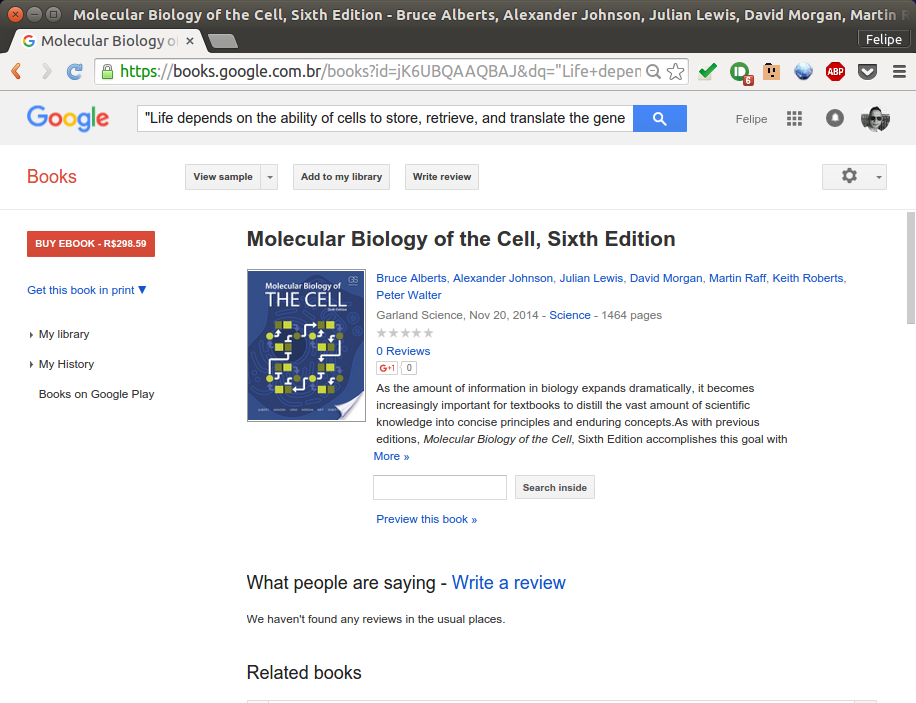
\includegraphics[height=.85\textheight]{Busca/gbooks-about1}
\end{frame}

\begin{frame}{Exportar arquivo RIS (RefMan)}
  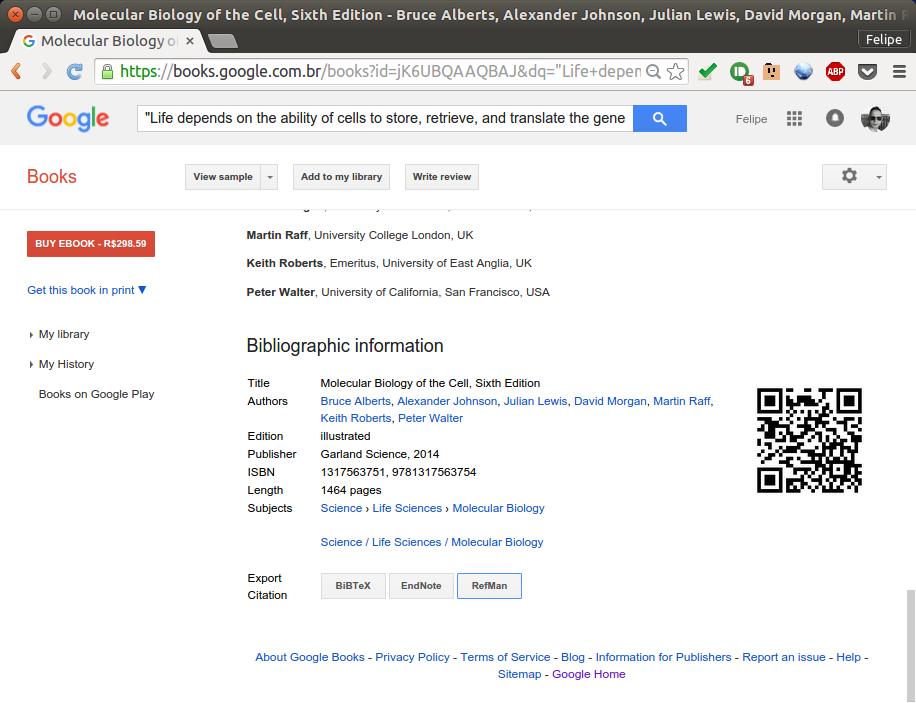
\includegraphics[height=.85\textheight]{Busca/gbooks-about2}
\end{frame}

\section{Deep Web}

\subsection{Papers}

\subsection{Livros}

\end{document}
